% !TEX program = xelatex

\documentclass[a4paper, 14 pt, titlepage]{extarticle}

\usepackage{grffile}
\usepackage{cmap}					% поиск в PDF
\usepackage[english,russian]{babel}	% локализация и переносы
\usepackage{indentfirst} 
\frenchspacing
\usepackage{setspace}
\usepackage{fontspec}      %% подготавливает загрузку шрифтов Open Type, True Type и др.
\defaultfontfeatures{Ligatures={TeX},Renderer=Basic}  %% свойства шрифтов по умолчанию
\setmainfont[Ligatures={TeX,Historic}]{Times New Roman} 
\setmonofont{Courier New}

\usepackage{amsmath,amsfonts,amssymb} 
\usepackage{amsthm}
\usepackage{mathtools}
\usepackage{icomma}

\renewcommand{\epsilon}{\ensuremath{\varepsilon}}
\renewcommand{\phi}{\ensuremath{\varphi}}
\renewcommand{\kappa}{\ensuremath{\varkappa}}
\renewcommand{\le}{\ensuremath{\leqslant}}
\renewcommand{\leq}{\ensuremath{\leqslant}}
\renewcommand{\ge}{\ensuremath{\geqslant}}
\renewcommand{\geq}{\ensuremath{\geqslant}}
\renewcommand{\emptyset}{\varnothing}

\usepackage{ragged2e}

\usepackage[unicode, pdfencoding=auto]{hyperref}
\usepackage[usenames,dvipsnames,svgnames,table,rgb]{xcolor}
\hypersetup{
            unicode=true,
            colorlinks=true,
            linkcolor=black,
            urlcolor=black,
            citecolor=black
           }

\usepackage{graphicx}
\graphicspath{{images/}}
\usepackage{wrapfig}
\usepackage{tikz}

\usepackage{listings}
\usepackage{color}

\lstset{
	basicstyle=\footnotesize\ttfamily,
	tabsize=4,
	columns=fixed,
	extendedchars=true,
	lineskip=-0.05\baselineskip,
	aboveskip=6pt,
	belowskip=6pt,
	breaklines,
	showstringspaces
}

\usepackage{cite}
\addto\captionsrussian{\renewcommand{\refname}{СПИСОК ИСПОЛЬЗОВАННЫХ ИСТОЧНИКОВ}}
\addto\captionsrussian{\renewcommand{\contentsname}{СОДЕРЖАНИЕ}}
\usepackage[titletoc]{appendix}
\addto\captionsrussian{\renewcommand{\appendixname}{Приложение}}
%\usepackage{tocloft}
%\usepackage{tocstyle}

\usepackage{array,tabularx,tabulary,booktabs, longtable, multirow}

\usepackage{etoolbox}
\usepackage{caption}
\captionsetup{labelsep=endash, font={singlespacing}, figurename=Рисунок }

\usepackage{lastpage}
\usepackage{fancyhdr} % Колонтитулы
 	\pagestyle{fancy}
 	\renewcommand{\headrulewidth}{0pt}  % Толщина линейки сверху
    \fancyfoot[R]{}
    \fancyfoot[C]{\thepage}
    \fancyhead[R]{}
    \fancyhead[L]{}
    
\setstretch{1.5}

\usepackage{extsizes}
\usepackage{geometry}
\geometry{top=2cm}
\geometry{bottom=2cm}
\geometry{left=3cm}
\geometry{right=1.5cm}

\usepackage{titlesec}

\renewcommand{\thesection}{\arabic{section}}
%\titleformat{\section}{\centering\normalsize \normalfont \bfseries }{\thesection}{1ex}{~\\\centering}[]
\titleformat{\section}{\centering\normalsize\normalfont\bfseries\uppercase}{\thesection.}{0.7ex}{}

\renewcommand{\thesubsection}{\thesection.\arabic{subsection}}
\titleformat{\subsection}{\normalsize\normalfont \bfseries}{\thesubsection.}{0.7ex}{}
\titlespacing\subsection{1.25cm}{1cm}{0pt}

\renewcommand{\thesubsubsection}{\thesubsection.\arabic{subsubsection}}
\titleformat{\subsubsection}{\normalsize\normalfont}{\thesubsubsection.}{0.7ex}{}
\titlespacing\subsubsection{1.25cm}{1cm}{0pt}

%\parindent=1.25cm
\setlength{\parindent}{1.25cm}

\newcommand{\startcode}{
    \footnotesize
    \singlespacing
}

\newcommand{\finishcode}{\setstretch{1.5}\normalsize}

\newenvironment{code}{\startcode}{\finishcode}

\newcommand{\printcaption}[1]{
    \normalsize
    {
    \captionsetup{justification=raggedright, singlelinecheck=off}
    \caption{#1}
    }
}




\newcommand{\subject}{Дифференциальные уравнения}
\newcommand{\theme}{Аппроксимация данных линейной комбинацией экспоненциальных функций}
\newcommand{\teacher}{Колоницкий С.Б.}
\newcommand{\studentn}{Поглазов Н.В.}
\newcommand{\studentr}{Цыганков Р.М.}
\newcommand{\groupnumber}{2384}
\newcommand{\group}{Группа 2384}

\begin{document}

\begin{titlepage}
   
   \begin{center}
       {
        \textbf{
             МИНОБРНАУКИ РОССИИ\\
             САНКТ-ПЕТЕРБУРГСКИЙ
             ГОСУДАРСТВЕННЫЙ
             ЭЛЕКТРОТЕХНИЧЕСКИЙ
             УНИВЕРСИТЕТ\\ <<ЛЭТИ>> ИМ.~
             В.И.~УЛЬЯНОВА (ЛЕНИНА)\\
            Кафедра МО ЭВМ\\
            \vspace{7cm}
            КУРСОВАЯ РАБОТА\\
            по дисциплине <<\subject>>\\
            Тема: \theme\\
        }
        
        \vspace{4cm}
        
       
       
       \setlength{\extrarowheight}{4mm}
       \begin{tabulary}{\textwidth}{LCCCL}
            Студент гр. \groupnumber & \hspace{0.5cm} & \hspace{4.5cm} & \hspace{0.5cm} & \student \\
            \cline{3-3}
            Преподаватель & \hspace{0.5cm} & \hspace{4.5cm} & \hspace{0.5cm} & \teacher \\
            \cline{3-3}
       \end{tabulary}
       \setlength{\extrarowheight}{0mm}
       
       \vfill
       
       Санкт-Петербург\\
       \the\year\\
       }
       
   \end{center}
   
  \end{titlepage}




\setcounter{page}{2}

\section*{Задание\\ на курсовую работу}

\setlength{\extrarowheight}{7mm}
\begin{tabularx}{\textwidth}{>{\raggedright\arraybackslash}X}
	Студент \studentn{} \studentr{}                                  \\
	\group                                                           \\
	Тема работы: \theme                                              \\
	Предполагаемый объём пояснительной записки: не менее 15 страниц. \\
	Дата выдачи задания: 17.10.2024                                  \\
	Дата сдачи реферата: 14.12.2024                                  \\
\end{tabularx}
\setlength{\extrarowheight}{0mm}

\vspace{50mm}
%\vfill

\setlength{\extrarowheight}{4mm}
\begin{tabulary}{\textwidth}{LCCCL}
	Студент & \hspace{0.5cm} & \hspace{4.5cm} & \hspace{0.5cm} & \studentn \\
	\cline{3-3}
	Студент & \hspace{0.5cm} & \hspace{4.5cm} & \hspace{0.5cm} & \studentr \\
	\cline{3-3}
	Преподаватель & \hspace{0.5cm} & \hspace{4.5cm} & \hspace{0.5cm} & \teacher \\
	\cline{3-3}
\end{tabulary}
\setlength{\extrarowheight}{0mm}

\newpage

\section*{АННОТАЦИЯ}
\begin{minipage}[t][0.4\textheight][t]{0.9\linewidth}
	\setlength{\parindent}{1.25cm}
	\indent
	В курсовой работе рассмотрена задача аппроксимации данных линейной комбинацией экспоненциальных функций. Основной целью исследования было разработать метод для нахождения оптимальных параметров модели с использованием алгоритма Левенберга-Марквардта. Были изучены математические основы метода, критерии сходимости и способы повышения численной устойчивости. Реализация алгоритма выполнена на языке Python с использованием библиотек NumPy и SciPy. Проведены эксперименты на сгенерированных данных, демонстрирующие эффективность предложенного подхода, а также влияние начальных приближений на качество решения. Разработанный метод подтвердил свою практическую применимость для задач анализа данных, что открывает перспективы для его дальнейшего улучшения и расширения.
\end{minipage}

\selectlanguage{english}
\section*{SUMMARY}
\begin{minipage}[t][0.4\textheight][t]{0.9\linewidth}
	\setlength{\parindent}{1.25cm}
	\indent
	The term paper addresses the problem of data approximation using a linear combination of exponential functions. The main objective of the study was to implement a method for finding the optimal model parameters using the Levenberg–Marquardt algorithm. The mathematical foundations of the method, convergence criteria, and approaches to enhancing numerical stability were examined. The algorithm was implemented in Python using the NumPy and SciPy libraries. Experiments on generated data demonstrated the efficiency of the proposed approach, as well as the influence of initial parameter estimates on the solution's quality. The developed method has proven its practical applicability to data analysis tasks, offering potential for further improvement and extension.
\end{minipage}
\selectlanguage{russian}

\newpage

\let \savenumberline \numberline
\def \numberline#1{\savenumberline{#1.}}

\tableofcontents

\newpage

\section*{Введение}
\addcontentsline{toc}{section}{Введение}

\subsection*{Цель работы.}

Разработка и реализация метода аппроксимации ряда данных линейной комбинацией экспоненциальных функций с неизвестными вещественными показателями.

\subsection*{Задание.}
Даны $(t_i, y_i)_{i=1}^n$, где $t_i \in \mathbb{R}$, $y_i \in \mathbb{R}$, $i = 1, \ldots, n$.

Рассмотрим $p$ — количество экспоненциальных членов, тогда мы подбираем функцию:
$$
	f: X \to Y; \:
	f(t, \textbf{p}) =\sum_{i=1}^p\lambda_i\alpha_i^t
$$
где $\textbf{p} = (\lambda_1, \ldots, \lambda_p, \alpha_1, \ldots, \alpha_p)$ — параметры, которые необходимо подобрать.

Предполагая, что $\forall i \:\alpha_i > 0$, можно переписать $f(t, \textbf{p})$ как:
$$
	f(t, \textbf{p})=\sum_{i=1}^p\lambda_i\exp(\ln(\alpha_i)t) =
	\sum_{i=1}^p\lambda_i\exp(\omega_it),
$$
где $\textbf{p} = (\lambda_1, \ldots, \lambda_p, \omega_1, \ldots, \omega_p)$

Функция потерь для оптимизации — это $\chi^2$, или взвешенный MSE, так как он часто используются в задачах аппроксимации кривых:
$$
	L(\mathbf{p}) = \chi^2(\boldsymbol p) = \sum_{i=1}^n\left(\frac{y_i-f(t_i, \boldsymbol p)}{\sigma_i}\right)^2 = \left[\mathbf y - \mathbf f\left ( \mathbf{p}\right )\right ]^T\boldsymbol{W}\left[\mathbf y - \mathbf f\left ( \mathbf{p}\right )\right ],
$$
где $\boldsymbol{W} = \operatorname{diag}\left(\frac{1}{\sigma_1^2}, \ldots, \frac{1}{\sigma_n^2}\right)$ - матрица весов: $\sigma_i^2=\mathbb{D}[y_i]$.

Метод оптимизации — алгоритм Левенберга-Марквардта, встроенный во множество библиотек для оптимизации, например, в SciPy.

\subsection*{Основные теоретические положения.}

Подобно другим численным методам минимизации, алгоритм Левенберга-Марквардта является итеративной процедурой. Для начала минимизации необходимо задать начальное приближение для вектора параметров. Начальное значение $\textbf{p}^T=\begin{pmatrix}1, 1, \dots, 1\end{pmatrix}$ подходит в большинстве случаев; в задачах с множеством локальных минимумов алгоритм сходится к глобальному минимуму, только если начальное приближение достаточно близко к решению.

На каждом шаге итерации вектор параметров $\textbf{p}$ заменяется новой оценкой $\textbf{p}+\boldsymbol{\Delta}$. Чтобы определить $\boldsymbol{\Delta}$, функция $f(t_i, \textbf{p} + \boldsymbol{\Delta})$ линеаризуется:
$$
	f(t_i, \textbf{p} + \boldsymbol{\Delta})\approx f(t_i, \textbf{p})+\mathbf{J}_i\boldsymbol{\Delta},
$$
где
\[
	\mathbf{J}_i = \frac{\partial f\left (t_i,  \mathbf{p}\right )}{\partial  \mathbf{p}}
\]

— это градиент $f$ по параметрам $\mathbf{p}$.

Таким образом, для текущей задачи $\forall j\le p:$
$$
	\mathbf{J}_{ij}=\frac{\partial f\left (t_i,  \mathbf{p}\right )}{\partial  \mathbf{\lambda_j}} = \exp(\omega_jt_i),
$$

$$
	\mathbf{J}_{ij+p}=\frac{\partial f\left (t_i,  \mathbf{p}\right )}{\partial  \mathbf{\omega_j}} = \lambda_jt_i\exp(\omega_jt_i).
$$

Функция потерь достигает минимума, когда её градиент по $\textbf{p}$ равен нулю. Для первого приближения $f\left (t_i,  \mathbf{p} + \boldsymbol\Delta\right )$:

$$
	L\left ( \mathbf{p} + \boldsymbol\Delta\right ) \approx \sum_{i=1}^n \left [\frac{y_i - f\left (t_i,  \mathbf{p}\right ) - \mathbf J_i \boldsymbol\Delta}{\sigma_i}\right ]^2
$$

или в векторной форме:

$$
	\begin{aligned}
		L\left ( \mathbf{p} + \boldsymbol\Delta\right ) & \approx \left [\mathbf y - \mathbf f\left ( \mathbf{p}\right ) - \mathbf J\boldsymbol\Delta \right ]^{\mathrm T}\boldsymbol{W}\left [\mathbf y - \mathbf f\left ( \mathbf{p}\right ) - \mathbf J\boldsymbol\Delta\right ]                                                                                                                                                              \\
		                                                & = \left [\mathbf y - \mathbf f\left ( \mathbf{p}\right )\right ]^{\mathrm T}\boldsymbol{W}\left [\mathbf y - \mathbf f\left ( \mathbf{p}\right )\right ] - 2\left [\mathbf y - \mathbf f\left ( \mathbf{p}\right )\right ]^{\mathrm T}\boldsymbol{W} \mathbf J\boldsymbol{\Delta} + \boldsymbol{\Delta}^{\mathrm T} \mathbf J^{\mathrm T} \boldsymbol{W} \mathbf J\boldsymbol{\Delta}.
	\end{aligned}
$$

Взяв производную от $L\left ( \mathbf{p} + \boldsymbol\Delta\right )$ по $\boldsymbol{\Delta}$ и приравняв её к нулю, получим:

$$
	\left (\mathbf J^{\mathrm T} \boldsymbol{W} \mathbf J \right ) \boldsymbol\Delta = \mathbf J^{\mathrm T}\boldsymbol{W}\left [\mathbf y - \mathbf f\left ( \boldsymbol p\right )\right ].
$$


Выражение выше соответствует методу Гаусса–Ньютона. Матрица Якоби $\mathbf{J}$ обычно не квадратная, а прямоугольная размерности $m \times n$, где $n$ — количество параметров. Перемножение $\mathbf J^{\mathrm T} \boldsymbol{W} \mathbf J$ дает квадратную матрицу размерности $n \times n$. Результат — это система из $n$ линейных уравнений, решаемая для $\boldsymbol{\Delta}$.

Вклад Левенберга заключается в использовании демпфированной версии уравнения:

$$
	\left (\mathbf J^{\mathrm T} \boldsymbol{W} \mathbf J + \lambda \mathbf{E} \right ) \boldsymbol\Delta = \mathbf J^{\mathrm T}\boldsymbol{W}\left [\mathbf y - \mathbf f\left ( \boldsymbol p\right )\right ].
$$

где $\lambda$ — коэффициент демпфирования, изменяемый после каждого вычисления $\boldsymbol{\Delta}$. Если снижение $L$ быстрое, значение $\lambda$ уменьшается, приближая алгоритм к методу Гаусса–Ньютона:

$$
	\boldsymbol{\Delta}\approx[\mathbf J^{\mathrm T} \boldsymbol{W} \mathbf J]^{-1}\mathbf{J}^{T}\boldsymbol{W}[\mathbf y - \mathbf f\left ( \mathbf{p}\right )],
$$

иначе $\lambda$ увеличивается, приближая шаг к направлению градиентного спуска:

$$
	\boldsymbol{\Delta}\approx\lambda^{-1}\mathbf{J}^{T}\boldsymbol{W}[\mathbf y - \mathbf f\left ( \mathbf{p}\right )].
$$

На старте алгоритма $\lambda$ обычно берется достаточно большим ($\approx 1$), чтобы делать первые шаги в направлении градиентного спуска. После каждой итерации $\lambda$ умножается или делится на определенный фактор, чтобы менять скорость сходимости.
Подробности см. в разделе "Выполнение работы"  подраздел "Детали реализации".

\newpage

\section{Выполнение работы}
\subsection{Детали реализации}

Так как производительность реализации, основанной исключительно на теоретических выкладках, оказалась недостаточной для практического применения, в итоговом решении были внесены несколько улучшений.

\subsubsection{Использование матрицы $\mathbf{W}$}

Поскольку мы имеем дело исключительно с синтетическими данными, и измерение $y_i$ проводятся единожды с заранее заданной (одинаковой) дисперсией, использование матрицы весов является избыточным. По этой причине в итоговой реализации $\mathbf{W} = \mathbf{E}$.

\subsubsection{Предобработка данных}

Для повышения численной устойчивости было принято решение стандартизировать данные перед обучением модели. Для этого используется формула:

\[
	x_i = \frac{x_i - \mu}{\sigma},
\]

то есть, после предобработки все значения признаков будут иметь нулевое среднее и единичное стандартное отклонение. Также этот метод не меняет форму распределения данных, что важно для сохранения интерпретируемости результатов.

\subsubsection{Обновление параметров}

Ранее, найденная $\boldsymbol{\Delta}$ применялась, если функция потерь уменьшалась, иначе она отклонялась, а коэффициент демпфирования увеличивался. Теперь шаг принимается, если метрика $\rho$ (была предложена Нильсеном в его статье 1999 года [3]) больше порогового значения $\epsilon_4 > 0$. Эта метрика измеряет фактическое уменьшение $\chi^2$ по сравнению с улучшением, достигаемым шагом метода Левенберга-Марквадта:

\[
	\begin{aligned}
		\rho & = \frac{\chi^2(\boldsymbol p) - \chi^2(\boldsymbol p + \boldsymbol\Delta)}
		{|(\boldsymbol{y}-\boldsymbol{\hat{y}})^T\mathbf{W}(\boldsymbol{y}-\boldsymbol{\hat{y}}) - (\boldsymbol{y}-\boldsymbol{\hat{y}}-\mathbf{J}\boldsymbol{\Delta})^T\mathbf{W}(\boldsymbol{y}-\boldsymbol{\hat{y}}-\mathbf{J}\boldsymbol{\Delta})|} \notag \\
		     & =\frac{\chi^2(\boldsymbol p) - \chi^2(\boldsymbol p + \boldsymbol\Delta)}
		{|\boldsymbol{\Delta}^T(\lambda\boldsymbol{\Delta} + \mathbf{J}^T\mathbf{W}(\boldsymbol{y}-\boldsymbol{\hat{y}}))|}\notag                                                                                                                              \\
	\end{aligned}
\]

где $\boldsymbol{\hat{y}} = \mathbf{f}(\boldsymbol{p})$.

Коэффициент демпфирования и параметры модели обновляются согласно следующим правилам:

Если $\rho > \epsilon_4$:
\[
	\lambda = \max\left[\frac{\lambda}{L_\downarrow},\:10^{-7}\right],\:\mathbf{p} \gets \mathbf{p} + \boldsymbol{\Delta}
\]
иначе:
\[
	\lambda = \min\left[\lambda L_\uparrow,\:10^{7}\right],\:\mathbf{p} \gets \mathbf{p}
\]

где $L_\downarrow\approx 9$ и $L_\uparrow\approx 11$ — фиксированные константы. Эти значения хорошо показали себя на практике и были выбраны на основе статьи [2].

\subsubsection{Критерии сходимости}

Алгоритм останавливается, когда выполняется \textit{одно} из следующих условий:

\begin{itemize}
	\item Сходимость по градиенту: $\operatorname{max}|\mathbf{J}^T\mathbf{W}(\boldsymbol{y}-\boldsymbol{\hat{y}})| < \varepsilon_1$
	\item Сходимость по коэффициентам: $\operatorname{max}|{\boldsymbol{\Delta}}/\mathbf{p}| < \epsilon_2$
	\item Сходимость по (редуцированному) $\chi^2$: $\chi^2_{\nu}=\chi^2/(m-n) < \epsilon_3$
\end{itemize}

\subsection{Программная реализация алгоритма}

Для реализации алгоритма был выбран язык программирования Python, так как он предоставляет широкие возможности для научных вычислений и имеет большое количество библиотек для работы с данными. В качестве основной библиотеки для работы с данными была выбрана библиотека NumPy, а для работы с графиками — Matplotlib.

\subsubsection{Структура проекта}

Проект разделен на следующие модули:

\begin{itemize}
	\item \texttt{exponential\_regression.py} — модуль с реализацией алгоритма в классе \texttt{ExponentialRegression}
	\item \texttt{loss/loss\_function.py} -- модуль с реализацией базового класса для функций потерь \texttt{LossFunction}
	\item \texttt{loss/chi2\_loss.py} -- модуль с реализацией функции потерь $\chi^2$ в классе \texttt{Chi2Loss}
	\item \texttt{main.py} — точка входа в программу, содержит пример использования алгоритма
\end{itemize}

\subsubsection{Класс \texttt{ExponentialRegression}}

Класс \texttt{ExponentialRegression} реализует регрессионную модель на основе экспоненциальных функций. Он наследует \texttt{BaseEstimator} и \texttt{RegressorMixin} из библиотеки \texttt{scikit-learn}, что делает его совместимым с её API. Основное назначение класса \texttt{ExponentialRegression}~--- обучение и предсказание на основе экспоненциальной зависимости.

При создании экземпляра класса задаются следующие параметры:
\begin{itemize}
	\item \texttt{n\_terms} (int, по умолчанию $1$): число экспоненциальных членов в модели.
	\item \texttt{max\_iter} (int, по умолчанию $1000$): максимальное число итераций для процедуры оптимизации.
	\item \texttt{gradient\_tol} (float, по умолчанию $10^{-3}$): порог для остановки оптимизации по величине градиента.
	\item \texttt{coefficients\_tol} (float, по умолчанию $10^{-3}$): порог для изменения коэффициентов модели.
	\item \texttt{chi2\_reduced\_tol} (float, по умолчанию $0.1$): порог для среднего значения $\chi^2$.
	\item \texttt{step\_acceptance} (float, по умолчанию $0.1$): минимальное значение отношения улучшения шага для принятия шага.
	\item \texttt{reg\_init} (float, по умолчанию $0.1$): начальное значение $\lambda$.
	\item \texttt{loss\_function} (\texttt{LossFunction}, по умолчанию \texttt{Chi2Loss}): функция потерь, используемая для вычисления градиента, гессиана и значения ошибки.
\end{itemize}

В дополнение к параметрам инициализации, класс определяет несколько предустановленных констант, $L\uparrow$ -- \texttt{REG\_INCREASE\_FACTOR}, \linebreak $L\downarrow$ -- \texttt{REG\_DECREASE\_FACTOR}, а также нижняя и верхняя граница $\lambda$ -- \texttt{REG\_MIN} и \texttt{REG\_MAX}.

\texttt{fit(data, target, initial\_lambda=None, \linebreak initial\_omega=None)}:

Метод обучает модель на основе входных данных:
\begin{itemize}
	\item \texttt{data} (\texttt{np.ndarray}): одномерный массив временных значений.
	\item \texttt{target} (\texttt{np.ndarray}): одномерный массив значений целевой переменной.
	\item \texttt{initial\_lambda} (\texttt{Optional[np.ndarray]}): начальные значения коэффициентов , если заданы.
	\item \texttt{initial\_omega} (\texttt{Optional[np.ndarray]}): начальные значения параметров , если заданы.
\end{itemize}
Для решения системы $[\mathbf{J}^T\mathbf{W}\mathbf{J}]\boldsymbol{\Delta}=\mathbf{J}^T\mathbf{W}(\mathbf{y}-\mathbf{\hat{y}})$ используется функция \linebreak \texttt{scipy.linalg.solve} из библиотеки SciPy.
\\*

\texttt{predict(data)}:

Метод делает предсказания для входных данных \texttt{data}:
\begin{itemize}
	\item \texttt{data} (\texttt{np.ndarray}): одномерный массив временных значений.
\end{itemize}

Приватные (вспомогательные) методы:

\begin{itemize}
	\item \texttt{\_init\_parameters(n\_terms)}: инициализация параметров $\mathbf{p}$.
	\item \texttt{\_jacobian(t)}: вычисление якобиана.
	\item \texttt{\_regularize\_hessian(hessian)}: демпфирование гессиана.
	\item \texttt{\_accept\_step(t, y\_true, y\_pred, delta, gradient)}: проверка, является ли шаг улучшением, и обновление параметров в случае успеха.
	\item \texttt{\_increase\_regularization()}: увеличение $\lambda$.
	\item \texttt{\_decrease\_regularization()}: уменьшение $\lambda$.
	\item \texttt{\_check\_convergence(gradient, lambda\_delta, omega\_delta, loss, measurements\_amount)}: проверка условий сходимости.
	\item \texttt{\_model(t, lambda\_=None, omega\_=None)}: вычисление $f(\mathbf{t}, \mathbf{p})$.
\end{itemize}


\subsubsection{Класс \texttt{Chi2Loss}}

Класс \texttt{Chi2Loss} реализует функцию потерь $\chi^2$. Он наследует \linebreak \texttt{LossFunction} и реализует методы для вычисления градиента, гессиана и значения функции потерь.

При создании экземпляра класса задаются следующие параметры:
\begin{itemize}
	\item \texttt{measurements\_amount} (\texttt{int}): количество измерений;
	\item \texttt{measurement\_variance} (\texttt{np.ndarray | float | None},  по умолчанию \texttt{None}): дисперсия каждого измерения или общая дисперсия;
\end{itemize}
с помощью которых вычисляется матрица весов $\mathbf{W}$.
\\*
\texttt{loss(y\_true, y\_pred)}:

Метод вычисляет значение функции потерь:
\[
	\chi^2 = \left[\mathbf y - \mathbf{\hat{y}}\right ]^T\mathbf{W}\left[\mathbf y - \mathbf{\hat{y}}\right ],
\]
\\*
\texttt{gradient(t, y\_true, y\_pred, jacobian)}:

Метод вычисляет (анти-) градиент функции потерь деленный на 2 (для удобства в использовании):
\[
	-\frac{1}{2}\frac{\partial\chi^2}{\partial\mathbf{p}} = \mathbf{J}^T\mathbf{W}(\mathbf{y}-\mathbf{\hat{y}})
\]
\\*
\texttt{hessian(jacobian)}:

Метод (приближенно) вычисляет гессиан функции потерь:

\[
	\frac{\partial^2\chi^2}{\partial\mathbf{p}^2} \approx \mathbf{J}^T\mathbf{W}\mathbf{J}
\]

где $\mathbf{\hat{y}}$ - \texttt{y\_pred},  $\mathbf{y}$ - \texttt{y\_true}, $\mathbf{J}$ - \texttt{jacobian}, $\mathbf{W}$ - диагональная матрица весов.

Реализованный код см. в приложении А, по ссылке: \url{https://github.com/Nekson228/ExponentialRegression/tree/main}, или по QR-коду:

\begin{figure}[h!]
	\centering
	
\includegraphics[width=0.2\linewidth]{../img/qr.png}
\end{figure}


\newpage
\section{Демонстрация работы программы}
\subsection{Пример с одним экспоненциальным членом}

Для примера были сгенерированы данные, соответствующие зависимости $f(t)=2\exp(-0.25t) + \epsilon,\:\epsilon\in\mathcal{N}(0, 1)$ — случайный шум.

Было проведено 100 замеров в диапазоне $t\in[-10, 10]$. После обучения модели были получены следующие результаты:

\begin{figure}[h!]
	\centering
	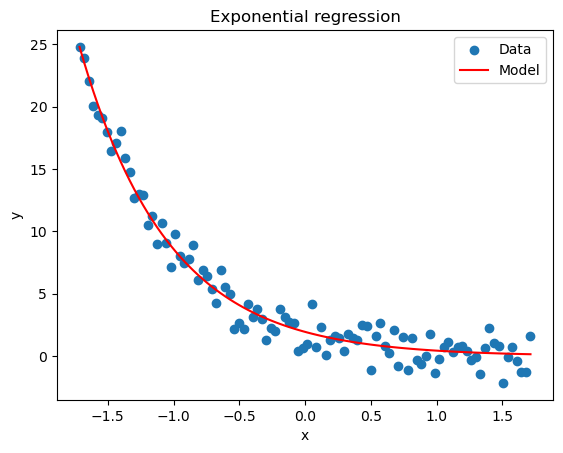
\includegraphics[width=0.7\linewidth]{../img/ex1.png}
	\caption{Пример с одним экспоненциальным членом}
\end{figure}

Как видно из графика, модель хорошо отфильтровала шум и восстановила исходную зависимость.

\subsection{Пример с двумя экспоненциальными членами}

Для примера были сгенерированы данные, соответствующие зависимости $f(t) = 2\exp(-0.25t)-5\exp(-2t)  + \epsilon,\:\epsilon\in\mathcal{N}(0, 0.1^2)$— случайный шум.

Было проведено 100 замеров в диапазоне $t\in[0, 10]$. После обучения модели были получены следующие результаты:

\begin{figure}[h!]
	\centering
	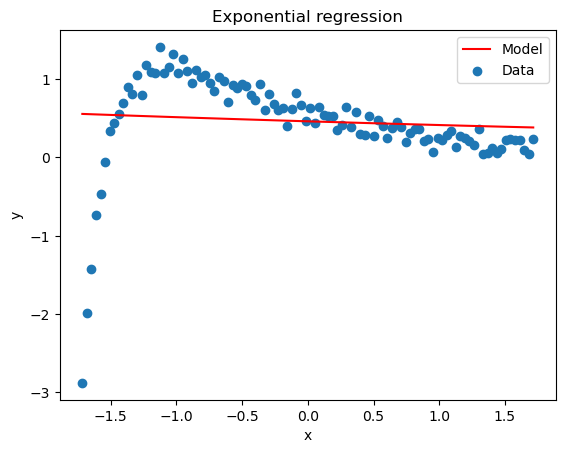
\includegraphics[width=0.7\linewidth]{../img/ex2_poor.png}
	\caption{Пример с двумя экспоненциальными членами}
	\label{fig:image}
\end{figure}

Как видно из графика, модель не смогла восстановить исходную зависимость. Это связано с тем, что функция потерь $\chi^2(\mathbf{p})$ может иметь множество локальных минимумов. В таких случаях метод Левенберга-Марквардта может сходиться к неудовлетворительному решению. Если это происходит, пользователь может попытаться задать лучшее начальное приближение для параметров, например, с помощью случайного поиска, или поиска по сетке, либо путем анализа данных.

Попробуем улучшить результат, вручную задав начальные приближения для параметров:
$$
	\begin{aligned}
		\boldsymbol{\lambda} & = \begin{bmatrix} 1 & -1 \end{bmatrix}  \\
		\boldsymbol{\omega}  & = \begin{bmatrix} -1 & -1 \end{bmatrix}
	\end{aligned}
$$

После обучения модели с новыми начальными приближениями были получены следующие результаты:

\begin{figure}[h!]
	\centering
	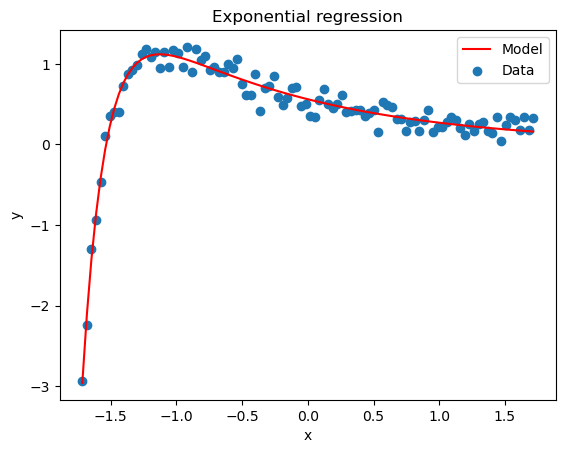
\includegraphics[width=0.7\linewidth]{../img/ex2_good.png}
	\caption{Пример с двумя экспоненциальными членами (улучшенный результат)}
\end{figure}


Как видно из графика, модель восстановила исходную зависимость. Это показывает, что правильный выбор начальных приближений для параметров может существенно повлиять на результат.

Написанный алгоритм позволяет удобно и быстро решать задачи аппроксимации данных линейной комбинацией экспоненциальных функций. Он легко расширяется на случай большего числа экспоненциальных членов, а также на случай других функций потерь.

\subsection{Примеры с не экспоненциальными зависимостями}

Попробуем провести подгон параметров модели к зависимостям, не являющимся линейной комбинацией экспоненциальных членов.

\newpage
\section*{Заключение}
\addcontentsline{toc}{section}{Заключение}

В процессе выполнения курсовой работы была достигнута цель, заключающаяся в разработке метода аппроксимации данных линейной комбинацией экспоненциальных функций с использованием алгоритма Левенберга-Марквардта. Были детально изучены основные математические принципы алгоритма, включая оптимизационные подходы, такие как градиентный спуск и метод Гаусса–Ньютона, а также особенности их сочетания в демпфированном виде.

Важным этапом стало внедрение методов повышения численной устойчивости, включая стандартизацию данных и адаптивное управление коэффициентом демпфирования. Реализованная модель продемонстрировала свою эффективность на тестовых данных, успешно аппроксимируя зависимости с одним и двумя экспоненциальными членами. Тем не менее, результаты также выявили чувствительность метода к выбору начальных приближений параметров, что требует дополнительного внимания при его применении.

Практическая реализация была выполнена на языке программирования Python с использованием современных библиотек для численных вычислений и визуализации. Предложенный подход может быть расширен для решения более сложных задач, например, с увеличением числа экспоненциальных членов или использованием других функций потерь. Разработанный алгоритм и полученные результаты подчеркивают его потенциал для дальнейших исследований и применения в задачах анализа данных.

\newpage

\addcontentsline{toc}{section}{Список использованных источников}
\begin{thebibliography}{99}
	\bibitem{wiki}
	Wikipedia contributors.
	\emph{Levenberg--Marquardt algorithm}.
	Wikipedia, The Free Encyclopedia.
	\url{https://en.wikipedia.org/wiki/Levenberg%E2%80%93Marquardt_algorithm}.

	\bibitem{gavin2020}
	H.~P. Gavin.
	\emph{The Levenberg-Marquardt algorithm for nonlinear least squares curve-fitting problems}.
	2020.
	\url{https://people.duke.edu/~hpgavin/ce281/lm.pdf}.

	\bibitem{nielson1999}
	H.~B. Nielsen.
	\emph{Damping Parameter in Marquardt's Method}.
	1999.
	\url{https://www2.imm.dtu.dk/documents/ftp/tr99/tr05_99.pdf}.
\end{thebibliography}

\newcommand{\sectionset}{\centering\normalsize\normalfont\bfseries\expandafter\uppercase}
\titleformat{\section}{\centering\normalsize\normalfont\bfseries}{}{0ex}{ПРИЛОЖЕНИЕ \thesection\\\uppercase}{}
\begin{appendices}
	\renewcommand{\thesection}{\Asbuk{section}}

	\newpage
	\section{Исходный код программы}

	\subsection{exponential\_regression.py}
	\lstinputlisting[language=Python]{../src/exponential_regression.py}

	\newpage
	\subsection{loss/loss\_function.py}
	\lstinputlisting[language=Python]{../src/loss/loss_function.py}

	\newpage
	\subsection{loss/chi2\_loss.py}
	\lstinputlisting[language=Python]{../src/loss/chi2_loss.py}

	\newpage
	\subsection{main.py}
	\lstinputlisting[language=Python]{../main.py}

\end{appendices}
\end{document}
